% Created 2024-11-14 Thu 15:28
% Intended LaTeX compiler: pdflatex
\documentclass[12pt]{article}
\usepackage[utf8]{inputenc}
\usepackage[T1]{fontenc}
\usepackage{graphicx}
\usepackage{longtable}
\usepackage{wrapfig}
\usepackage{rotating}
\usepackage[normalem]{ulem}
\usepackage{amsmath}
\usepackage{amssymb}
\usepackage{capt-of}
\usepackage{hyperref}
\usepackage[margin=1in]{geometry} \usepackage{amsmath} \usepackage{lipsum}
\author{Jason Press}
\date{\today}
\title{Physical Pendulums}
\hypersetup{
 pdfauthor={Jason Press},
 pdftitle={Physical Pendulums},
 pdfkeywords={},
 pdfsubject={},
 pdfcreator={Emacs 29.4 (Org mode 9.7.11)}, 
 pdflang={English}}
\begin{document}

\maketitle
\begin{abstract}


In this lab, we used a physical pendulum to calculate \(g\). We derived an equation to calculate \(g\) using the period, length, and distance from the center of mass to the axis of rotation. Then, after measuring the period for different distances using a photogate, we obtained an average value of \(g = 0.723\pm0.216\) m/s\textsuperscript{2}.
\end{abstract}
\section{Introduction}
\label{sec:org14e673c}

In this lab, we used a physical pendulum to measure \(g\). In order to do this, we measured the period and the moment of inertia of the pendulum. We can use the formula for the period of a physical pendulum to derive an equation for \(g\):

\begin{align*}
T = 2\pi\sqrt{\frac{I}{Mgx}} \implies g = \frac{4\pi^2 I}{MT^2x}
\end{align*}

Then, using the parallel-axis theorem, we can substitute \(I\) with \(M \left( \frac{L^2}{12} + x^2 \right)\) to arrive at an equation for \(g\) that relies only on the period \(T\), the length of the rod \(L\), and the displacement from the center of the rod to the axis of rotation \(x\):

\begin{align}
g = \frac{4\pi^2}{MT^2x} \left( \frac{L^2}{12} + x^2 \right)
\end{align}
\section{Methods}
\label{sec:org8b43170}

First, we measured the length of the rod with a meterstick. Our rod had holes in it, which we would use as the axis of rotation, so we measured the length from the base of the rod to the holes that we used. To get \(x\), we subtracted the distance from the base of the rod to the hole from half of the length of the rod.

To turn the rod into a physical pendulum, we put a small stick through the hole that we wanted to be the axis of rotation such that the rod could freely rotate about the stick.

To measure the period, we used a photogate set in pendulum mode. We made sure the bottom of the pendulum would pass through the photogate during its swing. To record a measurement, we set the photogate active, picked an arbitrary (but not large) height to release the pendulum from (since \(\theta\) does not change the period of a pendulum for \(\theta \lessapprox 15^{\circ}\)), and let the physical pendulum complete a full cycle through the photogate.

We performed ten trials at five different values of \(x\).

\begin{center}
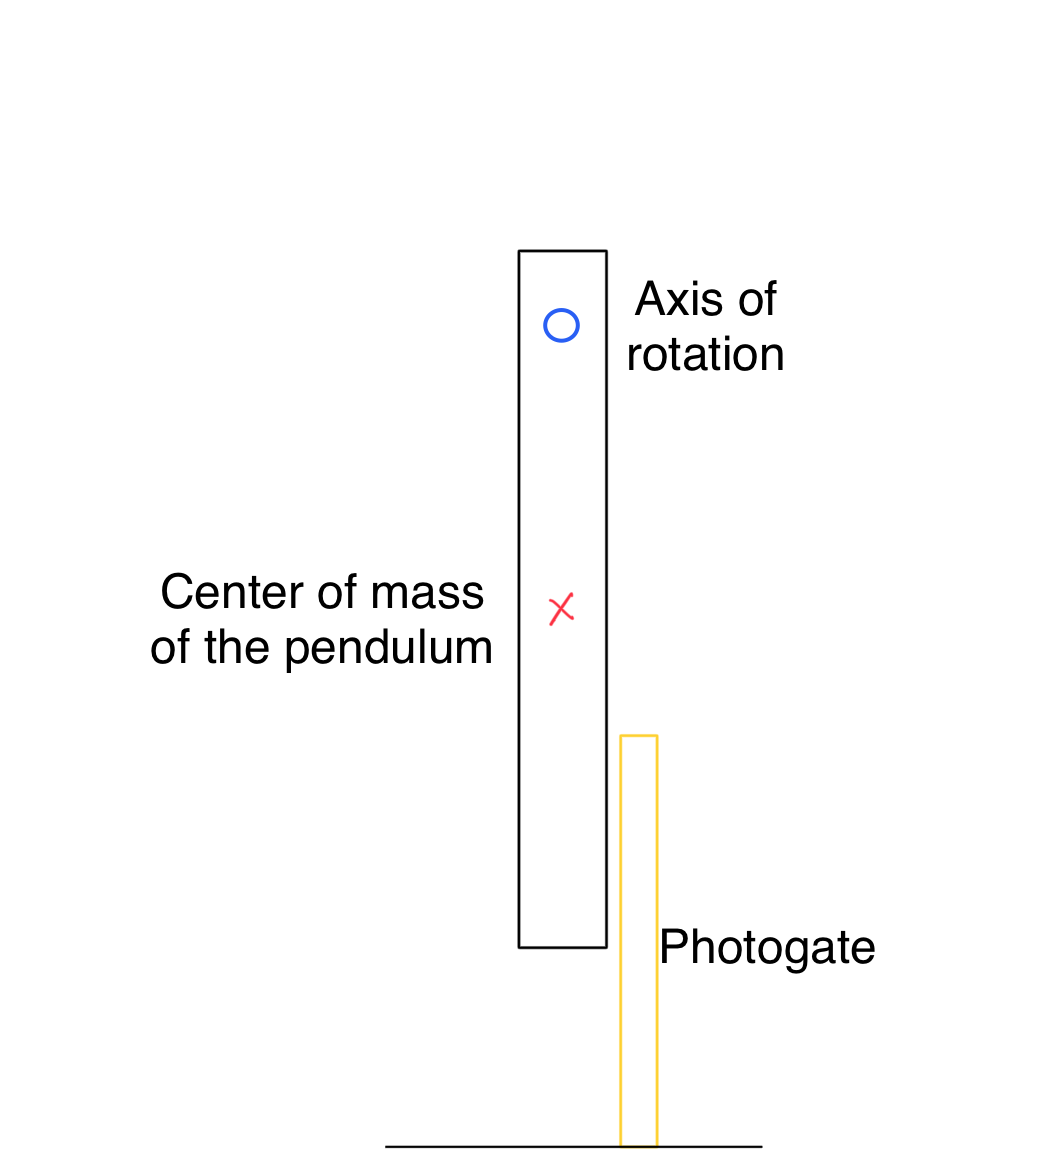
\includegraphics[height=7in]{./setup.png}
\captionof{figure}{Experimental setup}
\end{center}
\section{Results}
\label{sec:orgff6785a}

We measured our rod to be 1.118m long. Here are our results:

\begin{center}
\captionof{table}{Results}
\begin{tabular}{c|ccccc|}
Trial & Period  (s) &  &  &  & \\
\hline
\(x\) (m) & 0.500 & 0.452 & 0.406 & 0.361 & 0.320\\
\hline
1 & 1.6947 & 1.6676 & 1.6367 & 1.6230 & 1.6175\\
2 & 1.6951 & 1.6604 & 1.6429 & 1.6251 & 1.6148\\
3 & 1.6892 & 1.6635 & 1.6416 & 1.6236 & 1.6179\\
4 & 1.6890 & 1.6660 & 1.6401 & 1.6209 & 1.6220\\
5 & 1.6946 & 1.6697 & 1.6351 & 1.6264 & 1.6287\\
6 & 1.6957 & 1.6616 & 1.6428 & 1.6206 & 1.6243\\
7 & 1.6935 & 1.6672 & 1.6345 & 1.6148 & 1.6276\\
8 & 1.6939 & 1.6634 & 1.6377 & 1.6194 & 1.6274\\
9 & 1.6944 & 1.6645 & 1.6341 & 1.6236 & 1.6303\\
10 & 1.6957 & 1.6668 & 1.6413 & 1.6231 & 1.6329\\
\end{tabular}
\end{center}

This gave us an average \(g\) of 9.723\textpm{}0.216 m/s\textsuperscript{2}. This value contains \(g\).
\section{Discussion}
\label{sec:org066cf64}

Our main sources of error in this lab came from measuring \(x\). Although we determined the meterstick to have no statistical error for measuring \(L\), since repeated measurements yielded the same value of \(L\), we had a 1mm deviation within our group for measuring each \(x\). As such, we set our statistical error to half of 1mm, or 0.0005m. Otherwise, the resolution and systematic error for our use of the meterstick was 0.0005m, since the most amount of unnoticeable error we would introduce into the measurement with a meterstick is 0.0005m.

For our statistical error for \(T\), we used the standard deviation of all of the measurements. Just like for the meterstick, we set the resolution error for the photogate equal to the systematic error to the photogate.
\section{Sample Calculations}
\label{sec:org5796f9a}

We used a spreadsheet for all of our calculations. To get the position of the center of mass, we used \texttt{=A3/2}. To get \(x\), we used \texttt{=B3-A15}. To calculate \(g\) for one measurement, we used \texttt{=4*PI()\textasciicircum{}2/C2\textasciicircum{}2/B6*(A3\textasciicircum{}2/12+B6\textasciicircum{}2)}. Then, to obtain an average, we used \texttt{=AVERAGE(C17:C26,E17:E26,G17:G26,I17:I26,K17:K26)}. To get the actual error for a measurement \(\sigma\)\textsubscript{\(m\)}, we used \texttt{=sqrt(C31\textasciicircum{}2+D31\textasciicircum{}2+E31\textasciicircum{}2)}. For the error for one measurement, we used the following equation:

\begin{verbatim}
=sqrt((-8*PI()^2/C2^3*B6)^2*B31^2+(8*PI()^2*A3/12*C2^2*B6)^2*H31^2+
     (-8*PI()^2*A3^2/12*C2^2*B6^2+4*PI()^2/B6)^2*(M31)^2)
\end{verbatim}

Finally, to get the average \(\sigma\), we used \texttt{=AVERAGE(B43:B52,D43:D52,F43:F52,H43:H52,J43:J52)}.

Here is the spreadsheet we used. It's a bit of an unorganized mess since we have repeated values to make automation easier.

\begin{center}
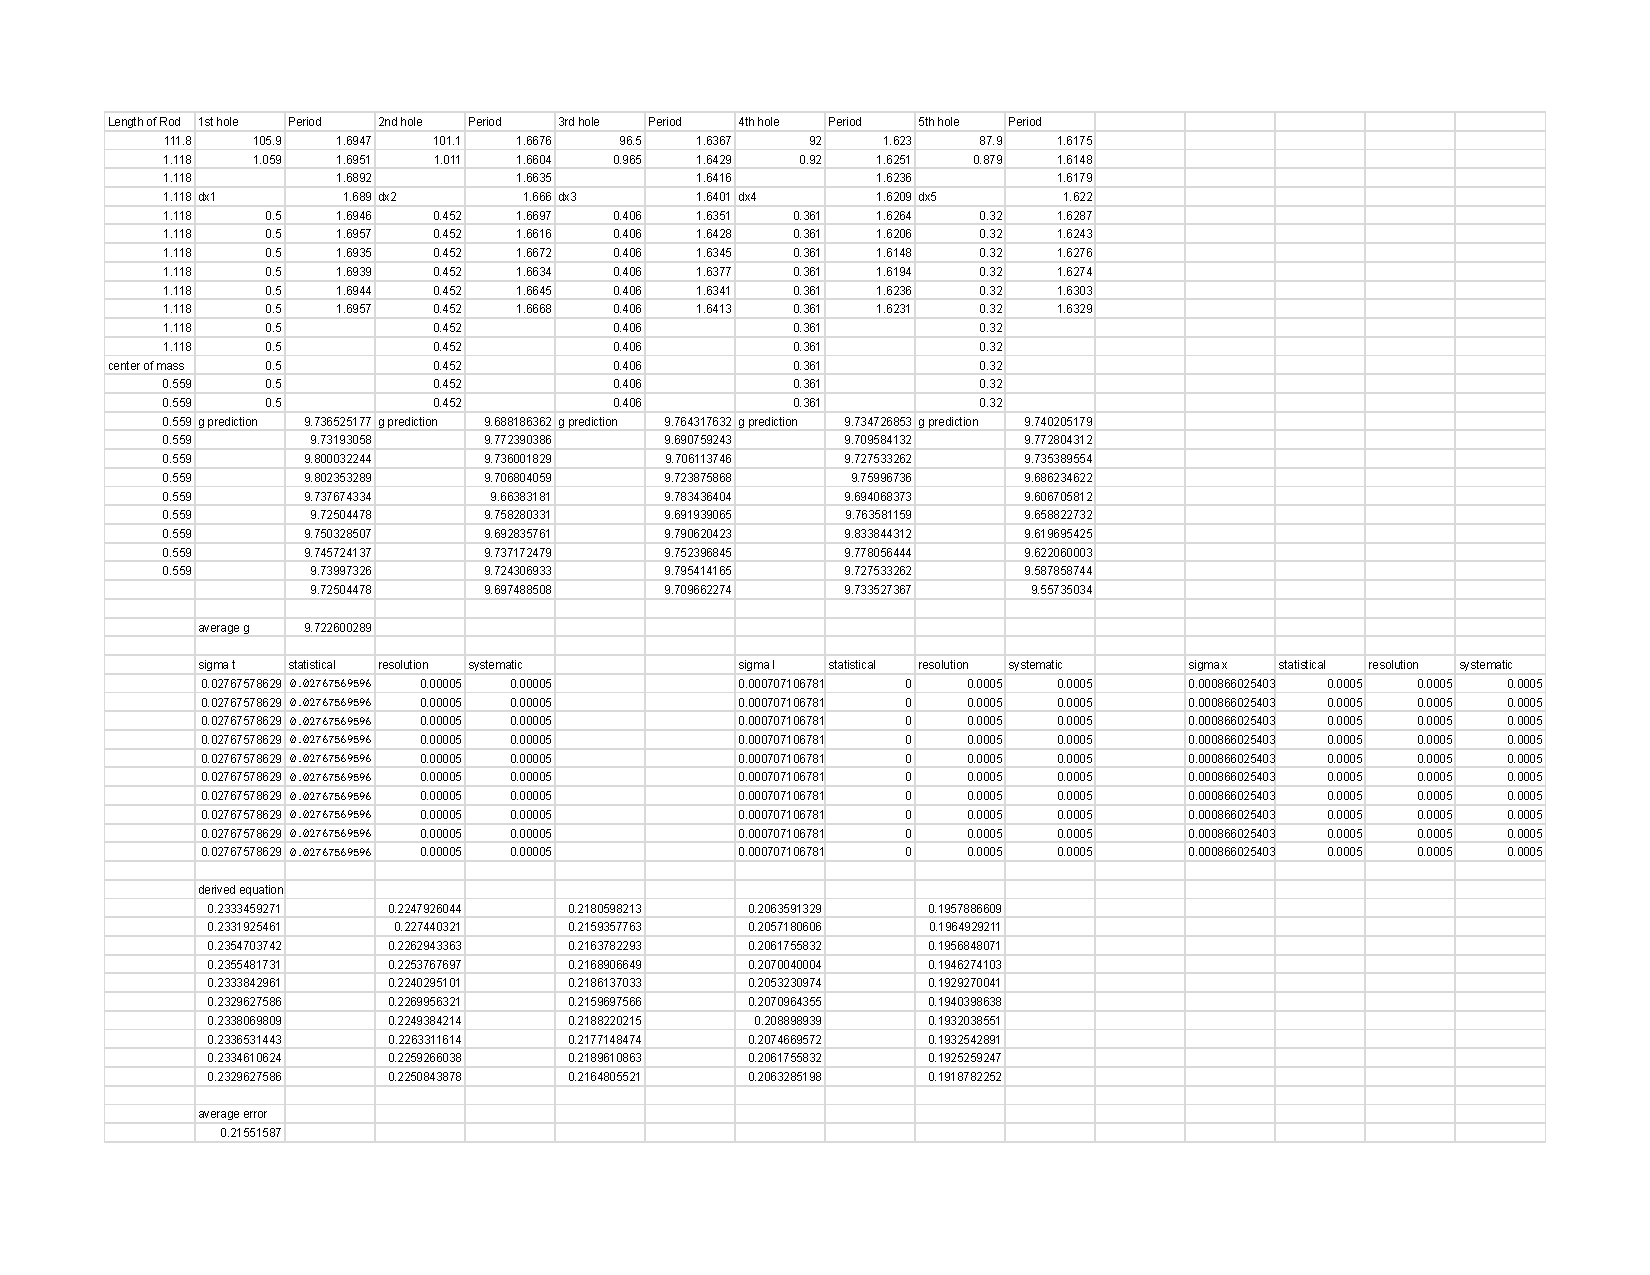
\includegraphics[width=7in]{./spreadsheet.pdf}
\end{center}
\end{document}
